%======================================================================
% T18_canon.pdf
%======================================================================
\section{Cvičení: Kanonický soubor}
\strana{T18-1}

\begin{veta}[Kuchařka ke kanonickému souboru]
\begin{enumerate}[label=\arabic*)]
  \item $H(p,q)$ \& fázový prostor
  \item $Z_c(\beta,V,N) = \displaystyle\int\dd\Gamma_N\,e^{-\beta H(p,q)}$
        \hfill $\dfrac{1}{N!}$\,? \dots\ extenzivita $F$
  \item $F(T,V,N) = \textcolor{Red}{\boxed{-\dfrac1\beta}}\log Z_c(\beta,V,N)\Big/_{\beta = \frac{1}{k_BT}}$
  \item termodynamika \dots \quad $S = -\Big(\dfrac{\partial F}{\partial T}\Big)_{V,N}$, \dots
  \item[4b)] $U = \langle H\rangle = -\dfrac{\partial\log Z_c}{\partial\beta}$ \quad \& \quad
        $\langle(\Delta H)^2\rangle = \dfrac{\partial^2\log Z_c}{\partial\beta^2}$
\end{enumerate}
\end{veta}

\noindent\rule{\linewidth}{0.4pt}

\begin{priklad}[Příklad 1 -- Dvouhladinový systém]
$N \gg 1$ nezávislých částic, každá se může nacházet ve
\[
  \ket{0} \leftrightarrow \epsilon_0 = 0, \qquad \ket{1} \leftrightarrow \epsilon_1 = \epsilon
\]
a) $S(T,V,N)$ \qquad b) $C(T)$
\end{priklad}

\[
  Z_c = \sum_{\text{stavy}}e^{-\beta H} \qquad H = \sum_{i=1}^{N}H_1(i) \qquad H_1 = \ket{0}0\bra{0} + \ket{1}\epsilon\bra{1}
\]
stavy $\updownarrow$ $\{n_1,\dots,n_N\}$, \quad $n_i \to 0$ nebo $1$
\[
  e^{-\beta H} = \prod_i e^{-\beta H_1(i)} \qquad
  \sum_{\text{stavy}} = \sum_{i=1}^{N}\sum_{j=0}^{1}
  \qquad \vzorec{Z_c = \prod_{i=1}^{N}Z_1 = (Z_1)^N}
\]
\pozn{v originále $e^{\beta H_1(i)}$ bez znaménka minus a $\sum_{\text{stavy}}$ zapsáno jako $\sum_i\sum_j$ místo součinu přes $i$}
\begin{align*}
  \sum_{i=1}^{2}\sum_{j_i=0}^{1} &= e^{-\beta(0+0)} + e^{-\beta(\epsilon+0)} + e^{-\beta(0+\epsilon)} + e^{-\beta(\epsilon+\epsilon)} \\
  &= e^{-\beta 0}\big(e^{-\beta0} + e^{-\beta\epsilon}\big) + e^{-\beta\epsilon}\big(e^{-\beta0} + e^{-\beta\epsilon}\big) \\
  &= \underbrace{\big(e^{-\beta0} + e^{-\beta\epsilon}\big)}_{Z_{i=2}}\underbrace{\big(e^{-\beta0} + e^{-\beta\epsilon}\big)}_{Z_{i=1}}
\end{align*}

%----------------------------------------------------------------------
\strana{T18-2}
$\bullet$ \kw{faktorizace partiční funkce} \\
\quad pro nezávislé stupně volnosti je \ $Z_c = \prod_i Z_i$
\[
  Z_1 = \sum_{\text{1-část.\ stavy}}e^{-\beta H} = e^{-\beta0} + e^{-\beta\epsilon} = 1 + e^{-\beta\epsilon}
\]
\[
  Z_c = \big(1 + e^{-\beta\epsilon}\big)^N \ \Rightarrow\ F(\beta,V,N) = -k_B\log Z_c = -Nk_B\log\big(1 + e^{-\beta\epsilon}\big)
\]
\pozn{v originále chybí faktor $T$: $F = -k_BT\log Z_c$}
\begin{align*}
  U = \langle H\rangle &= -\frac{\partial}{\partial\beta}\log Z_c = -N\frac{\partial}{\partial\beta}\log\big(1 + e^{-\beta\epsilon}\big)
  \qquad\qquad 0\cdot p(0) + \epsilon\,p(\epsilon) \\
  &= -\frac{N}{1 + e^{-\beta\epsilon}}\cdot\big(-\epsilon e^{-\beta\epsilon}\big) = N\frac{\epsilon e^{-\beta\epsilon}}{1 + e^{-\beta\epsilon}}
   = N\epsilon\,p(\epsilon)
\end{align*}
\hfill $\bra{1}\frac{1}{Z_c}e^{-\beta H}\ket{1} = \dfrac{e^{-\beta\epsilon}}{1 + e^{-\beta\epsilon}}$

\[
  \overset{\text{mikro}}{\boxed{E = \frac{N\epsilon}{1 + e^{\epsilon/k_BT}}}}
  \qquad C = \frac{\partial U}{\partial T} = \dots\ \text{Schottky}
\]

$\bullet$ \kw{záporné teploty:} \quad $\dfrac1T = \dfrac{\partial S}{\partial E}$

\begin{minipage}{0.5\textwidth}
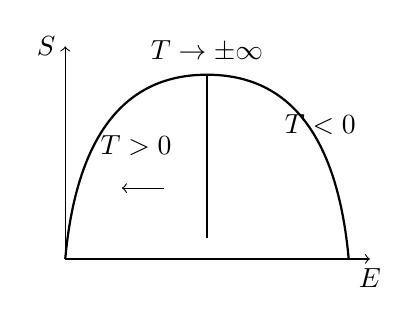
\begin{tikzpicture}[scale=0.9]
  \draw[->] (0,0) -- (4.3,0) node[below] {$E$};
  \draw[->] (0,0) -- (0,3) node[left] {$S$};
  \draw[thick] (0,0) .. controls (0.2,2.2) and (1.2,2.6) .. (2,2.6)
               .. controls (2.8,2.6) and (3.8,2.2) .. (4,0);
  \draw (2,2.6) -- (2,0.3);
  \node[above] at (2,2.65) {$T\to\pm\infty$};
  \node at (1,1.6) {$T > 0$};
  \draw[->] (1.4,1.0) -- (0.8,1.0);
  \node at (3.6,1.9) {$T < 0$};
\end{tikzpicture}
\end{minipage}
\begin{minipage}{0.45\textwidth}
rezervoár $\leftrightarrow$ nekonečný systém \\[4pt]
\hspace*{1.5cm}\pozor{$T > 0$\,!}
\end{minipage}

\noindent\rule{\linewidth}{0.4pt}

\subsection*{Ideální plyn kanonicky}
\begin{itemize}
  \item $H = \displaystyle\sum_{i=1}^{N}H_1 = \sum_{i=1}^{N}\frac{\vec p_i^{\,2}}{2m}$
\end{itemize}
\[
  Z_c = \int\dd\Gamma_N\,e^{-\beta H} = \frac{1}{N!}\int\prod_{i=1}^{N}\frac{\dd^3p_i\,\dd^3q_i}{h^3}\,
  \underbrace{e^{-\beta\sum_j\frac{p_j^2}{2m}}}_{=\prod_je^{-\beta\frac{p_j^2}{2m}}}
  = \frac{1}{N!}\Big(\int\frac{\dd^3p\,\dd^3q}{h^3}\,e^{-\beta\frac{p^2}{2m}}\Big)^N
\]
\[
  \Rightarrow\ \vzorec{Z_c = \frac{1}{N!}(Z_1)^N} \quad \uparrow \text{ faktorizace partiční funkce}
\]
\hfill \textcolor{Red}{$E = \displaystyle\sum_{i=1}^{3N}\frac{p_i^2}{2m} + \sum_{i<j}\phi(q_i,q_j)$}

%----------------------------------------------------------------------
\strana{T18-3}
\begin{align*}
  Z_1 &= \frac{1}{h^3}\int\underbrace{\dd^3q}_{\to V}\dd^3p\,e^{-\beta\frac{p^2}{2m}}
       = \frac{V}{h^3}\int\dd^3p\,e^{-\beta\overbrace{\scriptstyle p^2}^{= p_x^2 + p_y^2 + p_z^2}/2m}
       = \Big/\text{sfér.\ souřadnice}\Big/ \\
  &= \frac{4\pi V}{h^3}\int_0^\infty\dd p\,p^2e^{-\beta\frac{p^2}{2m}}
     = \Big/\ p\sqrt{\tfrac{\beta}{2m}} = x,\quad \dd p = \dd x\sqrt{\tfrac{2m}{\beta}}\ \Big/ \\
  &= \frac{4\pi V}{h^3}\sqrt{\frac{2m}{\beta}}^{\,3}\int_0^\infty\dd x\,x^2e^{-x^2}
\end{align*}
\[
  Z_1 = \frac{V}{h^3}\Big(\underbrace{\int_{-\infty}^{\infty}\dd p_i\,e^{-\frac{\beta}{2m}p_i^2}}_{\sqrt{\frac{2m\pi}{\beta}}}\Big)^3
  = \frac{V}{h^3}\Big(\frac{2\pi m}{\beta}\Big)^{3/2} = V\Big(\frac{2\pi m}{h^2\beta}\Big)^{3/2}
\]
\[
  Z_c = \frac{1}{N!}(Z_1)^N = \frac{1}{N!}V^N\Big(\frac{2\pi m}{h^2\beta}\Big)^{\frac{3N}{2}}
  \qquad \big(\tfrac1\beta = (k_BT)\big)^{3/2}
\]
\begin{align*}
  \Rightarrow\ F = -k_BT\log Z_c &= -Nk_BT\log\Big[V\beta^{-3/2}\Big(\frac{2\pi m}{h^2}\Big)^{3/2}\Big]
     + \underbrace{\log N!}_{+N\log N - N} \\
  &= -Nk_BT\log\Big(T^{3/2}\Big(\frac VN\Big)\Big)
     \underbrace{- \frac32Nk_B\log\Big(\frac{2\pi mk_B}{h^2}\Big) - N}_{Nf_0}
\end{align*}
\pozn{v originále u $\log N!$ chybí faktor $k_BT$}
\[
  \textcolor{Red}{\vzorec{F(T,V,N) = -Nk_BT\log\big(T^{3/2}VN^{-1}\big) + NTf_0}}
\]

\begin{minipage}{0.45\textwidth}
\color{Red}
$\underline{w(|\vec v| = v)} \sim e^{-\alpha v^2}$ \ $\swarrow E_k$

\medskip
$\bullet$ \ $S_\mu(T,V,N)$ vs.\ $S_c(T,V,N)$
\end{minipage}
\begin{minipage}{0.5\textwidth}
\color{Red}
Cv: \ $F(T,V,N)$ vč.\ $f_0$ v mikrokanon.\ formalismu
\end{minipage}

%----------------------------------------------------------------------
\strana{T18-4}
\subsection*{Ideální plyn v grav.\ poli}
\begin{minipage}{0.7\textwidth}
\[
  H = \sum_iH_1(i) \qquad
  H_1 = \frac{p^2}{2m} + \overset{\textcolor{NavyBlue}{F}}{mg}z \textcolor{NavyBlue}{\ = \frac{p^2}{2m} + Fz}
  \textcolor{Red}{\ = H_0 + H_I}
\]
\textcolor{Red}{$E = \langle H\rangle = U + \langle H_I\rangle$ \qquad $U = \langle H_0\rangle$}
\end{minipage}
\begin{minipage}{0.28\textwidth}
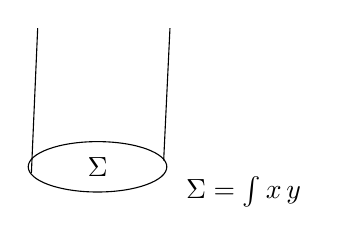
\begin{tikzpicture}[scale=0.8]
  \draw (0.1,2.6) -- (0,0.3);
  \draw (2.2,2.6) -- (2.1,0.5);
  \draw (1.05,0.4) ellipse (1.1 and 0.4);
  \node at (1.05,0.4) {$\Sigma$};
  \node[right] at (2.3,0.0) {$\Sigma = \int\dd x\,\dd y$};
\end{tikzpicture}
\end{minipage}

\[
  Z_c = \frac{1}{N!}(Z_1)^N
\]
\[
  Z_1 = \frac{1}{h^3}\int\dd^3p\,\dd^3q\,e^{-\beta H_1} = \Sigma\Big(\frac{2\pi m}{h^2\beta}\Big)^{3/2}\int_0^\infty\dd z\,e^{-\beta mgz}
\]
\hspace*{2cm}$\big(\sqrt{2\pi mk_BT} = \lambda_T$ \dots\ termální vlnová délka$\big)$ \pozn{tj.\ $\lambda_T = h/\sqrt{2\pi mk_BT}$}
\[
  = \Sigma\Big(\frac{2\pi m}{h^2\beta}\Big)^{3/2}\,\frac{e^{-\beta mgz}}{\beta mg}\Big|_\infty^0
  = \boxed{\Sigma\Big(\frac{2\pi m}{h^2}\Big)^{3/2}\beta^{-5/2}\frac{1}{mg} = Z_1}
\]
\[
  \Rightarrow\ F = -\frac1\beta\log Z_c = -\frac N\beta\log Z_1 + \frac1\beta\underbrace{\log N!}_{\sim N\log N - N}
\]
\[
  \boxed{F = -\frac N\beta\log\Big(\frac\Sigma N\beta^{-5/2}\Big) - \frac N\beta\log\Big[\Big(\frac{2\pi m}{h^2}\Big)^{3/2}\frac{1}{mg}\Big] - \beta N}
\]
\pozn{poslední člen správně $-N/\beta$}
\[
  \textcolor{Red}{\vzorec{F(T,\Sigma,N) = -Nk_BT\log\Big(T^{5/2}\frac\Sigma N\Big) - Nk_BT\log\Big[\frac{k_B^{5/2}}{mg}\Big(\frac{2\pi m}{h^2}\Big)^{3/2}\Big] - k_BTN}}
\]

\begin{minipage}{0.45\textwidth}
\[
  \boxed{w = \frac{1}{Z_c}e^{-\beta H_0 - \beta mgz}}
\]
\hspace*{1.2cm}$\downarrow$ \\
Legendre v TD potenciálu
\end{minipage}
\begin{minipage}{0.5\textwidth}
\textcolor{Red}{$G(T,\Sigma,\overset{\textcolor{NavyBlue}{F}}{mg},N)$}
\[
  \boxed{Z_c = \int\dd\Gamma_N\,e^{-\beta H_0 - \beta mgz}}
\]
\end{minipage}

\[
  S(U,V,N) \to S\Big[\frac1T\Big]\Big(\frac1T,\underset{\substack{\downarrow\\ x,y,z}}{V},N\Big)
  \qquad\text{pro } H = H_0 = \frac{p^2}{2m}
\]
\[
  \searrow\quad S\Big[\frac1T,\frac{F_z}{T}\Big]\Big(\frac1T,\frac{F_z}{T},y,x,N\Big)
\]
\[
  \langle z\rangle = \int\dd z\,z\,w = -\frac{1}{\beta m}\frac{\partial}{\partial g}\log Z_1
\]

%----------------------------------------------------------------------
\strana{T18-5}
\underline{Tepelná kapacita}
\[
  C_{\Sigma,N} = T\Big(\frac{\partial S}{\partial T}\Big)_{\Sigma,N} = -T\Big(\frac{\partial^2F}{\partial T^2}\Big)_{\Sigma,N}
\]
\[
  F(T,\Sigma,N) = -Nk_BT\log\Big(T^{5/2}\frac\Sigma N\Big)
  \ \textcolor{Red}{\underbrace{- Nk_BT\log\Big[\frac{k_B^{5/2}}{mg}\Big(\frac{2\pi m}{h^2}\Big)^{3/2}\Big] - k_BTN}_{\text{přeškrtnuto: } \frac{\partial^2}{\partial T^2} = 0}}
\]
\[
  \textcolor{Red}{F \simeq -Nk_BT\log T^{5/2}}
\]
\[
  \frac{\partial F}{\partial T} = -Nk_B\log T^{5/2} - \frac52Nk_B\frac TT \ \pozn{2.\ člen přeškrtnut}
  \qquad\qquad E = \langle H\rangle = \frac52Nk_BT
\]
\[
  \frac{\partial^2F}{\partial T^2} = -\frac52Nk_B\frac1T \ \Rightarrow\
  \vzorec{C_\Sigma = \frac52Nk_B} = \underset{\substack{\updownarrow\\ \text{kin.\ energie}}}{\frac32Nk_B} + \underset{\substack{\updownarrow\\ \text{grav.\ pole}}}{\frac22Nk_B}
\]
$C_V$ vs.\ $C_p$ \qquad $\swarrow$ \underline{\# kvadratických st.\ volnosti}\,! \qquad $T\nearrow$ \ $\langle z\rangle\nearrow$ \\
\hspace*{1cm}$c_V = \frac f2k_B$

$\langle z\rangle$:
\[
  \boxed{\Sigma\Big(\frac{2\pi m}{h^2}\Big)^{3/2}\beta^{-5/2}\frac{1}{mg} = Z_1}
  \qquad \langle z\rangle = \int\dd z\,z\,w = -\frac{1}{\beta m}\frac{\partial}{\partial g}\log Z_1
\]
\[
  \log Z_1 = -\log g + \log\Big(\Sigma\Big(\frac{2\pi m}{h^2}\Big)^{3/2}\beta^{-5/2}\frac1m\Big)
\]
\[
  \Rightarrow\ -\frac{1}{\beta m}\frac{\partial}{\partial g}\log Z_1 = \frac{1}{\beta mg}
  \ \Rightarrow\ \vzorec{\langle z\rangle = \frac{k_BT}{mg}} \quad \nearrow \text{ s } T \text{ roste lineárně}
\]
\[
  U = \langle H_0\rangle = \langle H\rangle - Nmg\langle z\rangle = \underset{\substack{\downarrow\\ \frac52Nk_BT}}{-\frac{\partial\log Z_c}{\partial\beta}} - Nk_BT
  \qquad (H = H_0 + mgz)
\]
